\documentclass[aspectratio=169,11pt]{beamer}
\usepackage{lmodern}
\usetheme[progressbar=frametitle,numbering=fraction]{metropolis}
\usepackage{amsmath,amssymb,bm}
\usepackage{listings,xcolor}
\usepackage{booktabs}
\definecolor{given}{HTML}{1F6FB2}
\definecolor{hand}{HTML}{2E7D32}
\definecolor{algo}{HTML}{B26A00}
\definecolor{impl}{HTML}{6A1B9A}
\lstset{language=Python,basicstyle=\ttfamily\footnotesize,keywordstyle=\color{impl}\bfseries,
  commentstyle=\color{gray},showstringspaces=false,columns=fullflexible,keepspaces=true}
% stage labels: every solution slide says which stage it is
\newcommand{\stage}[2]{{\color{#1}\bfseries\small\textsc{#2}}\par\smallskip}
\newcommand{\Byhand}{\stage{hand}{Step 1 -- by hand}}
\newcommand{\Algo}{\stage{algo}{Step 2 -- algorithm}}
\newcommand{\Impl}{\stage{impl}{Step 3 -- implementation}}
\newcommand{\Given}{\stage{given}{Recap}}

\title{Exercise 2 -- Problem 2.1: setting the stage}
\subtitle{Principles of Machine Learning (MA-INF 4111), WS 2026/27}
\date{Solution slides}
\begin{document}
\maketitle

\begin{frame}{Roadmap}
\begin{enumerate}
\item \textbf{Recap of the task}: what is given, which background we need, what we must do
\item \textbf{Task 2.1.1}: load and plot the myspace data
\item \textbf{Mini exercise}: show $f=\mathrm dF/\mathrm dt$ for the Weibull
\item \textbf{Task 2.1.2}: implement \texttt{weibull\_pdf()} and \texttt{weibull\_cdf()}
\end{enumerate}
\bigskip
Every solution follows the same three steps:\\[3pt]
\textcolor{hand}{\textbf{by hand}} \;$\to$\; \textcolor{algo}{\textbf{algorithm}} \;$\to$\; \textcolor{impl}{\textbf{implementation}}
\end{frame}

% =====================================================================
\section{Recap of the task}

\begin{frame}{Given: the myspace data}
\Given
\begin{columns}[T]
\column{.42\textwidth}
\begin{itemize}
\item File \texttt{dataMyspace201303.csv}, Google Trends, retrieved March 2013
\item One row per \textbf{week}: \\ \texttt{2004-07-11 - 2004-07-17,1}
\item Column 1: date range (text) \\ Column 2: search count (number)
\item Counts are \textbf{relative}: Google rescales so that the maximum is $100$
\end{itemize}
\column{.56\textwidth}
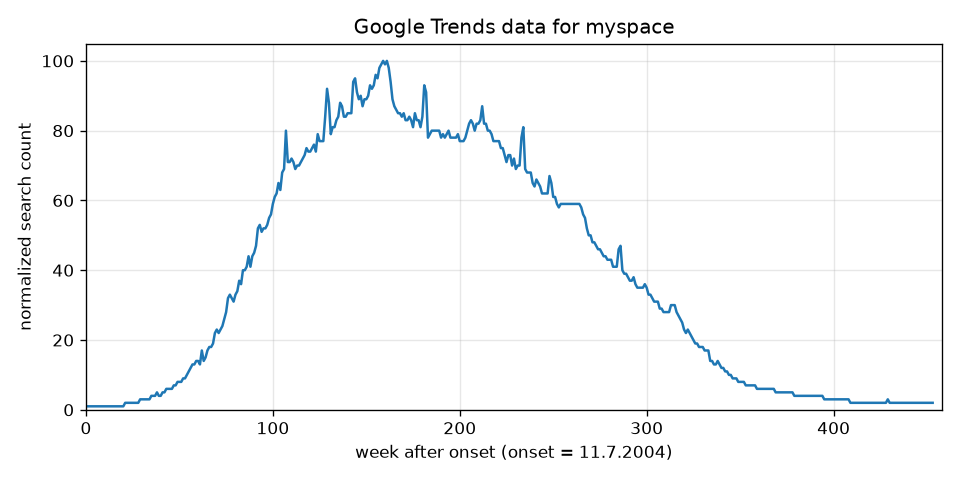
\includegraphics[width=\linewidth]{figures/task_2_1_1_data.png}
\end{columns}
\end{frame}

\begin{frame}{Background: why a Weibull?}
\Given
\begin{itemize}
\item The counts $c_t$ are a \textbf{histogram}: counts over discrete times $t$
\item Think of them as samples of an unknown (\emph{latent}) continuous density
\item The curve rises fast, peaks, then declines slowly $\Rightarrow$ \textbf{positively skewed}
\item A Gaussian is symmetric $\Rightarrow$ wrong model. We use the \textbf{Weibull}, $t\in[0,\infty)$:
\end{itemize}
\[
f(t\mid\alpha,\beta)=\frac{\alpha}{\beta}\Big(\frac t\beta\Big)^{\alpha-1}\exp\!\Big[-\Big(\frac t\beta\Big)^{\alpha}\Big]\quad(3)
\qquad
F(t\mid\alpha,\beta)=1-\exp\!\Big[-\Big(\frac t\beta\Big)^{\alpha}\Big]\quad(4)
\]
\begin{itemize}
\item $\alpha>0$: \textbf{shape},\quad $\beta>0$: \textbf{scale}
\end{itemize}
\end{frame}

\begin{frame}{Background: the Weibull describes rise and fall}
\Given
From (4): $\exp[-(t/\beta)^\alpha]=1-F(t)$. Insert this into (3):
\[
f(t)=\underbrace{\frac{\alpha}{\beta}\Big(\frac t\beta\Big)^{\alpha-1}}_{\text{growth term}}
\;-\;\underbrace{\frac{\alpha}{\beta}\Big(\frac t\beta\Big)^{\alpha-1}F(t)}_{\text{decline term}}\qquad(5)
\]
\begin{itemize}
\item Both terms are polynomial in $t$
\item $F(t)$ grows monotonically, so the decline term catches up over time
\item[$\Rightarrow$] the longer the process runs, the faster it declines: exactly the myspace story
\end{itemize}
\end{frame}

\begin{frame}{Problem to solve}\small
\Given
\begin{description}[Task 2.1.1]
\item[Task 2.1.1] Read column 2 into a numpy array, remove the \textbf{leading} zeros, call the rest
$\bm c=[c_1,\dots,c_n]$ and build $\bm t=[1,2,\dots,n]$ (start at $1$!). Plot $\bm c$ against $\bm t$.
Wrap both in reusable functions.
\item[Mini ex.] Using (3) and (4), show that $f=\dfrac{\mathrm dF}{\mathrm dt}$.
\item[Task 2.1.2] Implement (3) and (4) as numpy functions \texttt{weibull\_pdf()}, \texttt{weibull\_cdf()}
with explicit parameters $\alpha,\beta$. \textbf{Do not} use \texttt{scipy.stats}.
\end{description}
\end{frame}

% =====================================================================
\section{Task 2.1.1: load and plot the data}

\begin{frame}{2.1.1 -- by hand on a toy file}\small
\Byhand
Suppose column 2 of a tiny file reads
\[
\text{raw}=[\,0,\;0,\;0,\;1,\;3,\;0,\;2,\;5\,]
\]
\begin{enumerate}
\item First non-zero entry: position $4$ (value $1$). Three \textbf{leading} zeros.
\item Remove them: $\bm c=[1,\,3,\,0,\,2,\,5]$, so $n=5$.\\
\quad The zero \emph{inside} stays: it is a real measurement (a week with no searches).
\item Time steps: $\bm t=[1,2,3,4,5]$, \emph{not} $[0,\dots,4]$.
\item Plot the points $(t_i,c_i)$: $(1,1),(2,3),(3,0),(4,2),(5,5)$.
\end{enumerate}
\medskip
\alert{Why start at $t=1$?} Later we use $\log t$ and bins $(t_{j-1},t_j]$ with $t_0=0$; for $\alpha<1$ the density is infinite at $t=0$.
\end{frame}

\begin{frame}{2.1.1 -- the real file}
\Byhand
\begin{center}
\begin{tabular}{lr}
\toprule
rows in the file (weeks from 4.1.2004 to 16.3.2013) & $480$\\
leading zeros (4.1.2004 -- 10.7.2004) & $27$\\
remaining values $n$ & $480-27=453$\\
first week kept (onset) & 11.7.2004\\
$\max_t c_t$ & $100$ at $t=159$\\
zeros left inside $\bm c$ & none\\
\bottomrule
\end{tabular}
\end{center}
\medskip
Sanity checks: the onset matches the sheet (second week of July 2004), $n$ is ``slightly more than 400 weeks'', and the maximum is $100$ as Google's normalisation demands.
\end{frame}

\begin{frame}[fragile]{2.1.1 -- algorithm}
\Algo
\begin{enumerate}
\item Read column 2 of the csv as numbers: $\text{raw}_1,\dots,\text{raw}_N$
\item Find the first index with a positive value: $k=\min\{i:\text{raw}_i>0\}$
\item Keep everything from there on: $\bm c=[\text{raw}_k,\dots,\text{raw}_N]$, \;$n=N-k+1$
\item Build $\bm t=[1,\dots,n]$
\item Plot $\bm c$ over $\bm t$; label the axes ``week after onset'' and ``normalized search count''
\end{enumerate}
\medskip
\alert{Pitfall:} ``keep all $c_i>0$'' (a mask) would also delete interior zeros. We need ``cut off the front''.
\end{frame}

\begin{frame}[fragile]{2.1.1 -- implementation}
\Impl
\begin{columns}[T]
\column{.55\textwidth}
\begin{lstlisting}
def load_myspace_data(fname):
    raw = np.loadtxt(fname, delimiter=",",
                     usecols=1)   # column 2 only
    k = np.argmax(raw > 0)        # first True
    c = raw[k:]                   # cut the front
    t = np.arange(1, len(c) + 1)  # 1, ..., n
    return t, c

def plot_data(t, c):
    plt.plot(t, c)
    plt.xlabel("week after onset")
    plt.ylabel("normalized search count")
\end{lstlisting}
\column{.43\textwidth}
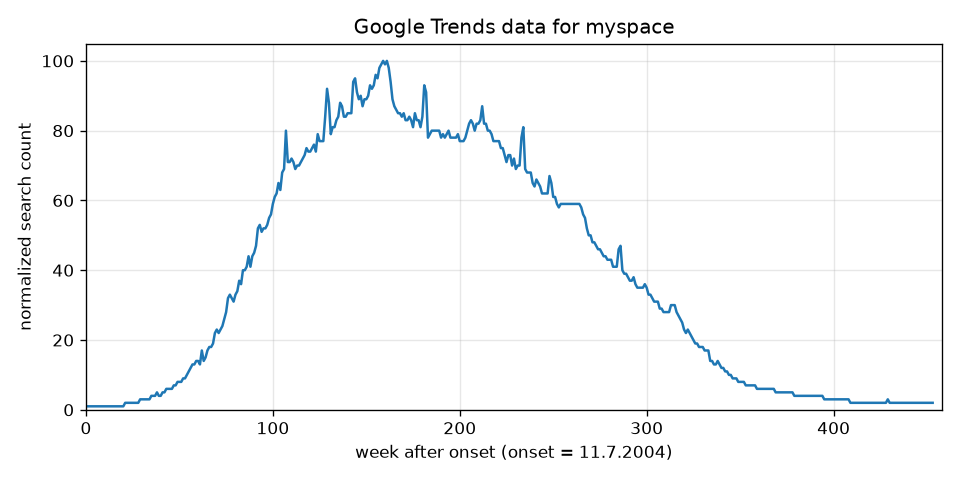
\includegraphics[width=\linewidth]{figures/task_2_1_1_data.png}
\small
\begin{itemize}
\item \texttt{usecols=1}: column 1 is text
\item \texttt{argmax} on booleans = first \texttt{True}
\end{itemize}
\end{columns}
\end{frame}

% =====================================================================
\section{Mini exercise: $f=\mathrm dF/\mathrm dt$}

\begin{frame}{Mini exercise -- by hand}
\Byhand
\textbf{Goal:} differentiate $F(t)=1-\exp[-(t/\beta)^\alpha]$ and get (3).
\begin{enumerate}
\item Name the inner function: $u(t)=\big(\tfrac t\beta\big)^{\alpha}$, so $F=1-e^{-u}$.
\item Derivative of $u$ (power rule, then inner factor $\tfrac1\beta$):
\[u'(t)=\alpha\Big(\frac t\beta\Big)^{\alpha-1}\cdot\frac1\beta\]
\item Chain rule: $\dfrac{\mathrm dF}{\mathrm dt}=0-e^{-u}\cdot(-u')=u'\,e^{-u}$
\item Insert:
\[\frac{\mathrm dF}{\mathrm dt}=\frac\alpha\beta\Big(\frac t\beta\Big)^{\alpha-1}\exp\!\Big[-\Big(\frac t\beta\Big)^{\alpha}\Big]=f(t\mid\alpha,\beta)\qquad\blacksquare\]
\end{enumerate}
\end{frame}

\begin{frame}{Mini exercise -- is $f$ a proper density?}
\Byhand
Because $f=F'$, the integral of $f$ is a difference of $F$-values:
\[
\int_0^\infty f(t)\,\mathrm dt=\lim_{t\to\infty}F(t)-F(0)
=\big(1-e^{-\infty}\big)-\big(1-e^{0}\big)=1-0=1
\]
(using $\alpha>0$, so $(t/\beta)^\alpha\to\infty$). Also $f\ge0$ everywhere.
\medskip
\begin{itemize}
\item[$\Rightarrow$] $f$ is a probability density, $F$ is its cumulative distribution
\item Typical mistake: forgetting the factor $\tfrac1\beta$ from the inner derivative
\end{itemize}
\end{frame}

\begin{frame}[fragile]{Mini exercise -- checking by computer}\small
\Algo
A derivation by hand can be checked in two independent ways:
\begin{enumerate}
\item \textbf{Symbolic:} let a computer algebra system compute $F'-f$ and simplify. Must give $0$.
\item \textbf{Numerical:} central difference $\dfrac{F(t+h)-F(t-h)}{2h}\approx f(t)$ for small $h$, at many $t$.
\end{enumerate}
\Impl
\begin{lstlisting}
t, a, b = sp.symbols("t alpha beta", positive=True)
F = 1 - sp.exp(-(t/b)**a)
f = a/b * (t/b)**(a-1) * sp.exp(-(t/b)**a)
sp.simplify(sp.diff(F, t) - f)        # -> 0
\end{lstlisting}
\small Numerically ($\alpha=2.5,\ \beta=200$, 50 points): largest error $9\cdot10^{-13}$; $\int_0^\infty f=1.0000$.
\end{frame}

% =====================================================================
\section{Task 2.1.2: \texttt{weibull\_pdf()} and \texttt{weibull\_cdf()}}

\begin{frame}{2.1.2 -- by hand: evaluate one point}
\Byhand
Take $\alpha=2,\ \beta=1,\ t=1$, so $t/\beta=1$:
\[
f(1\mid2,1)=\frac21\cdot1^{1}\cdot e^{-1^2}=2e^{-1}\approx0.736,
\qquad
F(1\mid2,1)=1-e^{-1}\approx0.632
\]
Special case $\alpha=1$: $f(t)=\tfrac1\beta e^{-t/\beta}$, the \textbf{exponential} distribution.
\medskip

These hand values become \textbf{test cases} for the code.
\end{frame}

\begin{frame}{2.1.2 -- by hand: what do $\alpha$ and $\beta$ do?}\small
\Byhand
\textbf{Scale $\beta$.} Write $s=t/\beta$. Then
\[f(t\mid\alpha,\beta)=\frac1\beta\,f\big(\tfrac t\beta\mid\alpha,1\big)\]
$\Rightarrow$ doubling $\beta$: curve twice as wide, half as high, area still $1$.

\textbf{Shape $\alpha$.} Where is the peak? Set $\frac{\mathrm d}{\mathrm dt}\log f=0$:
\[
\frac{\alpha-1}{t}-\frac{\alpha\,t^{\alpha-1}}{\beta^\alpha}=0
\;\Longrightarrow\;
t_{\text{mode}}=\beta\Big(\frac{\alpha-1}{\alpha}\Big)^{1/\alpha}\quad(\alpha>1)
\]
\begin{itemize}
\item $\alpha<1$: no peak, $f$ decreases and $f(0)=\infty$;\quad $\alpha=1$: exponential
\item $\alpha>1$: rises from $0$, one peak, then falls $\Rightarrow$ the myspace shape needs $\alpha>1$
\item Example $\alpha=2.5,\ \beta=2$: $t_{\text{mode}}=2\cdot0.6^{0.4}\approx1.63$
\end{itemize}
\end{frame}

\begin{frame}{2.1.2 -- algorithm}
\Algo
\begin{enumerate}
\item Inputs: times $t$ (a number or an array), shape $\alpha>0$, scale $\beta>0$
\item Compute $s=t/\beta$ elementwise
\item pdf: return $\frac\alpha\beta\,s^{\alpha-1}e^{-s^\alpha}$;\quad cdf: return $1-e^{-s^\alpha}$
\end{enumerate}
\medskip
Design choices:
\begin{itemize}
\item work elementwise on arrays (numpy broadcasting): one call evaluates the whole curve
\item $\alpha,\beta$ are explicit arguments, so later tasks can try many parameter values
\item $t=0$ with $\alpha<1$ gives $\infty$: mathematically correct, not a bug
\end{itemize}
\end{frame}

\begin{frame}[fragile]{2.1.2 -- implementation}
\Impl
\begin{lstlisting}
def weibull_pdf(t, alpha, beta):
    s = np.asarray(t, dtype=float) / beta     # works for numbers and arrays
    return alpha/beta * s**(alpha-1) * np.exp(-s**alpha)

def weibull_cdf(t, alpha, beta):
    s = np.asarray(t, dtype=float) / beta
    return 1.0 - np.exp(-s**alpha)

weibull_pdf(1, 2, 1)   # 0.7358  = 2/e      (our hand value)
weibull_cdf(1, 2, 1)   # 0.6321  = 1 - 1/e  (our hand value)
\end{lstlisting}
\small Extra check: agrees with \texttt{scipy.stats.weibull\_min(c=$\alpha$, scale=$\beta$)} up to $10^{-18}$ (used only as a test).
\end{frame}

\begin{frame}{2.1.2 -- the sheet's plots confirm the hand analysis}
\Impl
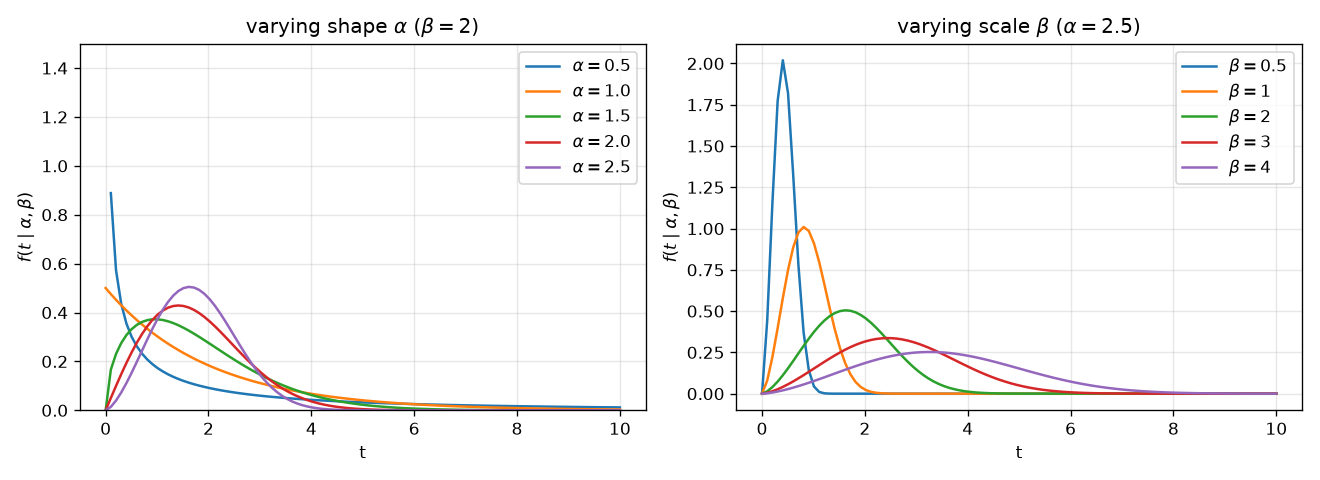
\includegraphics[width=\linewidth]{figures/task_2_1_2_shape_scale.png}
\small Left ($\beta=2$): $\alpha<1$ decreasing and infinite at $0$, $\alpha=1$ exponential, $\alpha>1$ one peak (for $\alpha=2.5$ at $1.63$).
Right ($\alpha=2.5$): larger $\beta$ = wider and lower, same area.
\end{frame}

% =====================================================================
\section{Takeaways}

\begin{frame}{Takeaways}
\begin{itemize}
\item Choose a model because it fits the data's \textbf{shape} (skewed rise and fall), not because it is easy
\item The Weibull has a built-in growth term minus a decline term, see (5)
\item $\alpha$ sets the form, $\beta$ only stretches time
\item Small details matter: $\bm t$ starts at $1$; remove only \emph{leading} zeros
\item The counts are relative (max $=100$): later methods must not depend on the absolute scale of $\bm c$
\item Check by hand, then by computer: symbolic, numerical, and against known values
\end{itemize}
\end{frame}

\end{document}
